\chapter{State of the Art}
% \thispagestyle{fancy}
\textit{In this chapter, a detailed description about background of the degree project is presented together with related work. This chapter reviews the current technological advances and identifies the research gaps in optimal control of soft quadruped robots and model-based reinforcement learning.}

Explain what and how prior work / prior research will be applied on or used in the degree project /work (described in this thesis). Explain why and what is not used in the degree project and give valid reasons for rejecting the work/research.

\section{Current Control of Soft Quadruped Robot}
 In comparison to rigid legs, which can be modeled using multi-body dynamics for their dynamic movements, soft legs with soft actuators are more challenging to be modeled and controlled than rigid legs due to their non-linearity\cite{slotineAppliedNonlinearControl1991} and time variant properties\cite{wangControlStrategiesSoft2022}, such as hysteresis and drift, where the high non-linearity of soft materials makes them difficult to predict and control, and the hysteresis and drift can also increase the occurrence of unpredictable behaviors. Furthermore, the need to consider continuum mechanics, which deals with the behavior of continuously deformable materials with infinite \ac{DoF}\cite{polygerinosSoftRoboticsReview2017}, adds an extra level of complexity. 

In general, the control to a soft robot still require further research to establish the internal connection with control science\cite{wangControlStrategiesSoft2022}. Typically, the loads of rigid legs are different between the two cases of leg suspension and stepping on the ground\cite{biswalDevelopmentQuadrupedWalking2021}, which means that the dynamics of the quadruped robot is a mixture of continuous and discrete, such that the model is continuous when touching the ground or when hovering, but there is a sudden change from hovering to touching the ground, which makes the model behave a discrete. In addition, because of the influence of external gravity, the force required to move the motor at the same angle is different for different leg suspension positions, so the leg model of the quadruped is nonlinear, so that it is common to use a model predictive controller for rigid quadruped robots. However, it is not easy to predict the behavior of a soft robot if using a model predictive controller\cite{BemporadLinearTimevaryingNonlinearMPC}, so it is desired to have more identical solutions for the controllers, whereby the  reinforcement learning came to our mind\cite{hewingLearningbasedModelPredictive2020}. 

\section{Model-based Reinforcement Learning}
As the complexity of robotics increases, \ac{RL} is increasingly required to develop robust control algorithms with high \ac{DoF}s and time variant properties\cite{zhangEffectiveSoftRobot2017}. The rapid development of AI provides an alternative solution to take into account the nonlinear properties of novel materials and soft robots\cite{tangModelbasedOnlineLearning2021}. \ac{MFRL} is a type of reinforcement learning where an agent learns to make decisions based on experiences and rewards obtained from the environment, without having an explicit model of the environment. The agent directly can map observations to actions, through trial and error, without considering the underlying dynamics of the environment\cite{arulkumaranDeepReinforcementLearning2017}. The goal of model-free reinforcement learning is to learn a policy $\Pi$, which is a mapping from states to actions, that maximizes the expected cumulative reward over time. The \ac{MBRL} refers to a type of \ac{RL} where an agent learns optimal behavior by learning a model of the environment by taking actions and observing the outcomes that include the next step and the immediate reward\cite{rayModelBasedReinforcementLearning2010}. 
\begin{figure}[hp]
    \centering
    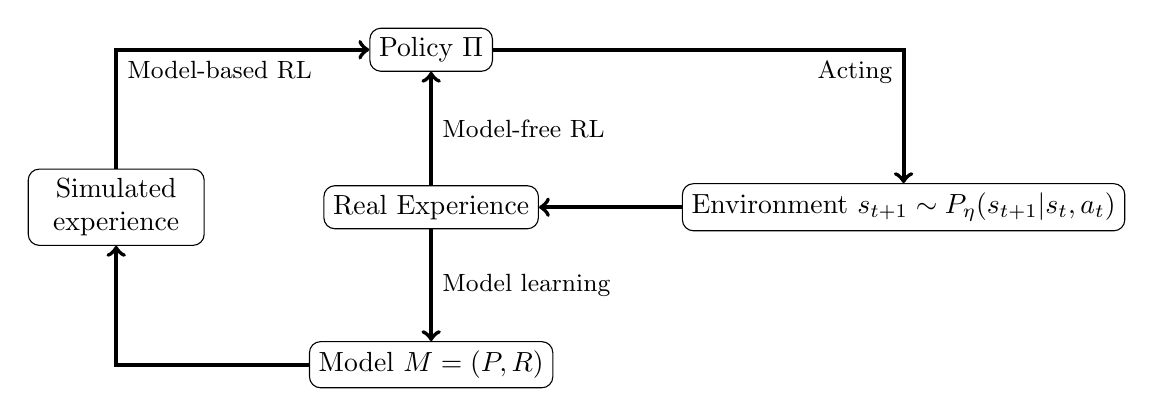
\begin{tikzpicture}[node distance=2cm]
        % Define nodes
        \node (policy) [rounded corners, draw] {Policy $\Pi$};
        \node (real_experience) [rounded corners, draw, below of=policy] {Real Experience};
        \node (environment) [rounded corners, draw, right of=real_experience, node distance=6cm] {Environment $s_{t+1}\sim P_\eta(s_{t+1}|s_t, a_t)$};
        \node (model) [rounded corners, draw, below of=real_experience] {Model $M = (P,R)$};
        \node (simulated_experience) [align=center, text width=2cm, rounded corners, draw, left of=real_experience, node distance=4cm] {Simulated experience};
        
        % Draw arrows
        \draw[->, line width=1.5pt] (policy) -| (environment) node[midway, below left, font=\small] {Acting};
        \draw[->, line width=1.5pt] (environment) -- (real_experience);
        \draw[->, line width=1.5pt] (real_experience) -- (model) node[midway, right, font=\small] {Model learning};
        \draw[->, line width=1.5pt] (model) -| (simulated_experience);
        \draw[->, line width=1.5pt] (real_experience) -- (policy) node[midway, right, font=\small] {Model-free RL};
        \draw[->, line width=1.5pt] (simulated_experience) |- (policy) node[font=\small, midway, below right] {Model-based RL};
    \end{tikzpicture}
    \caption{Model-free \ac{RL} vs. Model-based \ac{RL}}
    \label{fig:demo}
\end{figure}
% \tikzstyle{block} = [draw, fill=white, rectangle, 
%     minimum height=3em, minimum width=6em]
% \tikzstyle{sum} = [draw, fill=white, circle, node distance=1cm]
% \tikzstyle{input} = [coordinate]
% \tikzstyle{output} = [coordinate]
% \tikzstyle{pinstyle} = [pin edge={to-,thin,black}]

% \begin{tikzpicture}[auto, node distance=2cm,>=latex']

%     \node [input, name=input] {};
%     \node [sum, right of=input] (sum) {};
%     \node [block, right of=sum] (controller) {Controller};
%     \node [block, right of=controller, pin={[pinstyle]above:D},
%             node distance=3cm] (system) {System};

%     \draw [->] (controller) -- node[name=u] {$u$} (system);
%     \node [output, right of=system] (output) {};
%     \node [block, below of=u] (measurements) {Measurements};

%     \draw [draw,->] (input) -- node {$r$} (sum);
%     \draw [->] (sum) -- node {$e$} (controller);
%     \draw [->] (system) -- node [name=y] {$y$}(output);
%     \draw [->] (y) |- (measurements);
%     \draw [->] (measurements) -| node[pos=0.99] {$-$} 
%         node [near end] {$y_m$} (sum);
% \end{tikzpicture}

Typically, the model can be considered as a combination of state transition distribution $P_\eta$ and reward function $R_\eta$, $$M = (P,R) \textrm{ where } s_{t+1}\sim P_\eta(s_{t+1}|s_t, a_t) \textrm{ and } r_{t+1}\sim R_\eta(r_{t+1}|s_t, a_t)$$ $s_t$ is the state at time $t$, $r_t$ is the reward at time $t$ and $a_t$ is the action at time $t$. Model-based \ac{RL} learns an abstract model of the environment to plan the optimal policy. This model can be used to simulate the consequences of its actions, allowing it to make informed decisions, which makes it applicable to handle more complex environments, as it can make use of a model of the environment's dynamics. Therefore, model-based \ac{RL} requires a prior knowledge of the domainology\cite{tangModelbasedOnlineLearning2021}, as a model needs to be created and maintained. The domain of the model-based \ac{RL} refers to the context or environment in which the \ac{RL} agent is operating, which determines the available actions, observations, and rewards, and hence influences the behavior of the agent\cite{langExplorationRelationalDomains}. In model-based \ac{RL}, the agent needs to build a model of the dynamics of the system within the domain, and this model should accurately represent the true behavior of the system in order for the agent to learn effectively.
\section{Use headings to break the text}


\subsection{Related Work}

One approach to RL is model-based RL, where the agent learns a model of the environment dynamics and uses this model to plan its actions. Model-based RL has the potential to improve sample efficiency, which is crucial for robotics applications where data collection can be time-consuming and expensive. Model-based RL has been successfully applied to various robotics tasks, including manipulation and locomotion. However, the effectiveness of model-based RL depends on the accuracy of the learned model, which can be challenging to achieve in complex environments.

Several studies have investigated the use of model-based RL for quadruped robots. For example, Ha and Schmidhuber (2018) proposed an approach called world model-enhanced RL, where the agent learns a compact world model of the environment dynamics and uses it to plan its actions. They applied this approach to a simulated quadruped robot and achieved superior performance compared to other RL methods. Similarly, Chowdhary et al. (2020) proposed a model-based RL approach for quadruped robots that used a Gaussian process regression model to estimate the dynamics of the robot's locomotion. They demonstrated the effectiveness of their approach on a physical quadruped robot.

Soft robots have also been the subject of RL research. For example, Geijtenbeek et al. (2018) developed an RL-based controller for a soft robot arm that could grasp and manipulate objects. They used a model-free RL algorithm called deep deterministic policy gradient and demonstrated that the controller could adapt to different object shapes and sizes. Meanwhile, Yao et al. (2020) proposed a model-based RL approach for controlling a soft robotic arm with a cable-driven actuation system. They used a physics-based model of the arm and achieved superior performance compared to other RL methods.

Overall, the existing literature suggests that model-based RL has the potential to develop optimal policies for quadruped robots, including soft quadruped robots. However, the effectiveness of the approach depends on the accuracy of the learned model and the complexity of the environment. In addition, most existing studies have focused on simulated environments, and there is a need for further research on applying model-based RL to physical soft quadruped robots in real-world settings.
